Рассматривались 3 глобальных темы: обзор препятствий, роботы, которые используются в исследованиях пещер, а так же методы построения карты местности.

\subsection{Обзор
препятствий}

Для решения поставленной цели необходимо понимать в каких условиях будет использоваться робот.

Пещера -- полость в верхней части земной коры, сообщающаяся с поверхностью одним или несколькими входными отверстиями. Они бывают различных типов, от этого зависит какой набор препятствий будет встречаться чаще.

Основные структуры поверхностей следующие \pic{fig:obstacles}:
\begin{itemize}
    \item твердые породы, прочные -- мрамор, кварц, базальт (магма);
    \item твердые породы, мягкие -- мел, гипс, соль, известняк;
    \item сыпучие грунты -- песок, глина, снег;
    \item водные преграды -- как и лужи (малый слой воды), так и целы залы, погруженные под воду. Часто встречаются сифоны;
    \item скользкие поверхности -- отложения мха и плесени, лед ;
    \item разрушаемые поверхности -- каменная гряда, паутина.
\end{itemize}

\begin{figure}[ht]
    \begin{subfigure}[b]{0.3\textwidth}
        \centering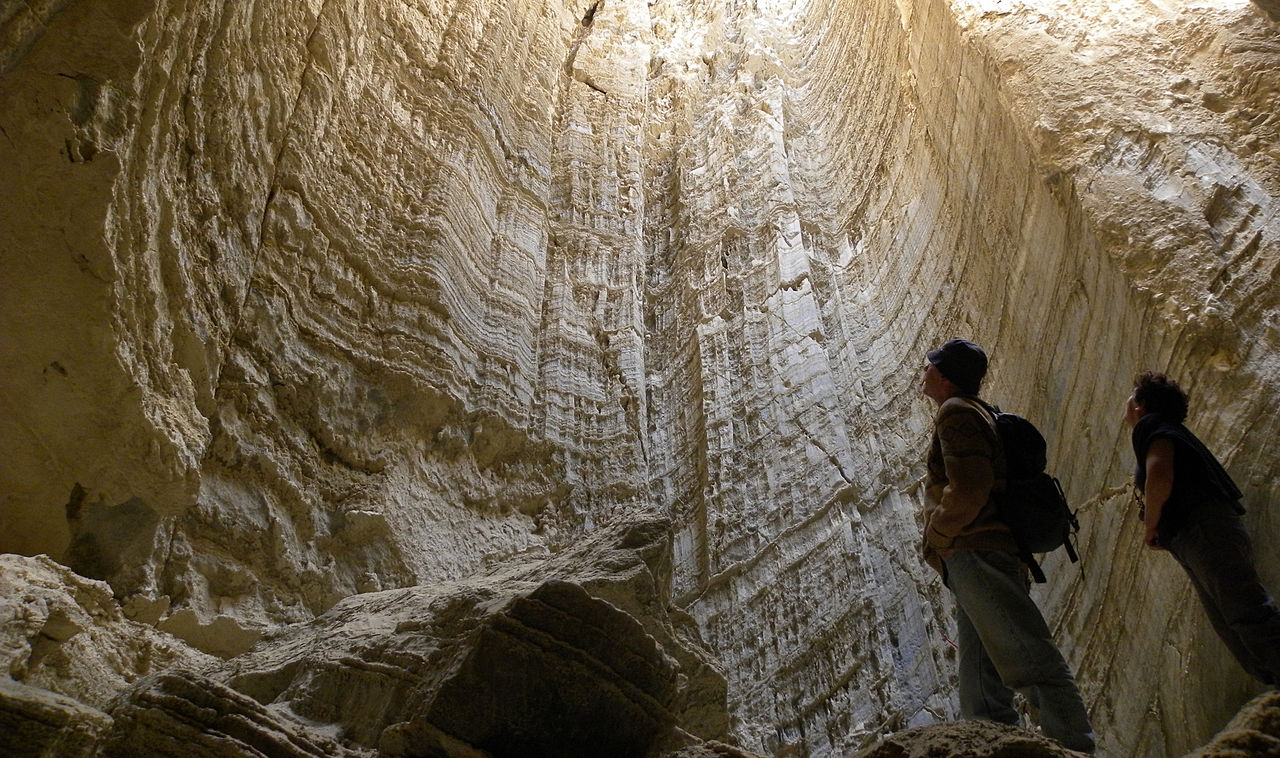
\includegraphics[height=2.8cm,width=1\textwidth,keepaspectratio]{surface_types/salt.jpg}\\
        \caption{Соляные отложения}
        \label{fig:surface_types/salt}
    \end{subfigure}
    \hfill
    \begin{subfigure}[b]{0.3\textwidth}
        \centering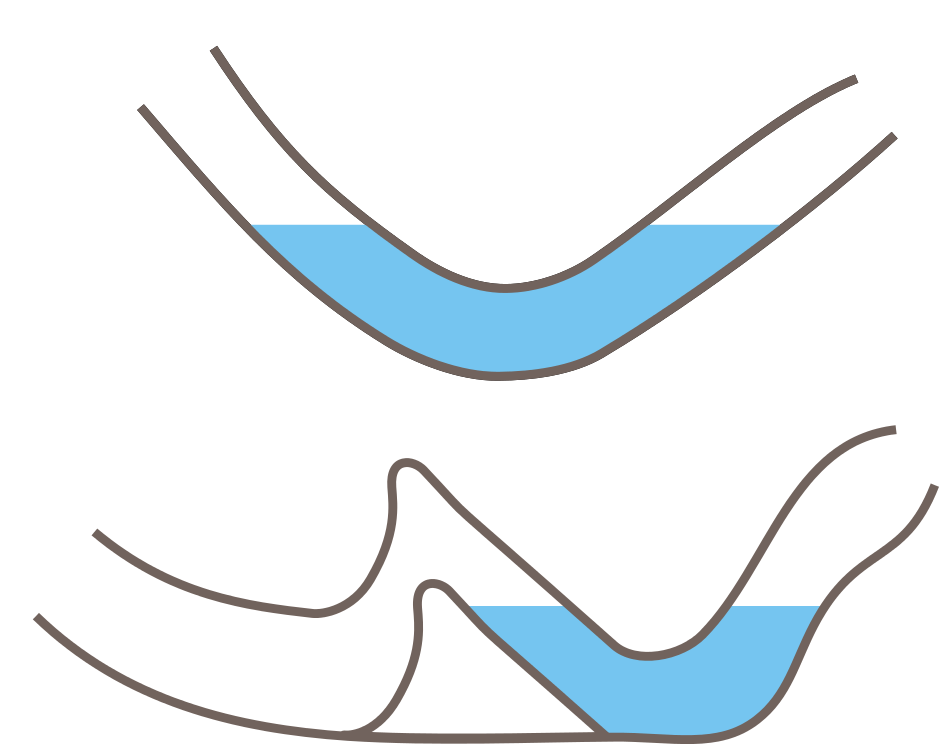
\includegraphics[height=2.8cm,width=1\textwidth,keepaspectratio]{surface_types/siphon.png}\\
        \caption{Сифон}
        \label{fig:surface_types/siphon}
    \end{subfigure}
    \hfill
    \begin{subfigure}[b]{0.3\textwidth}
        \centering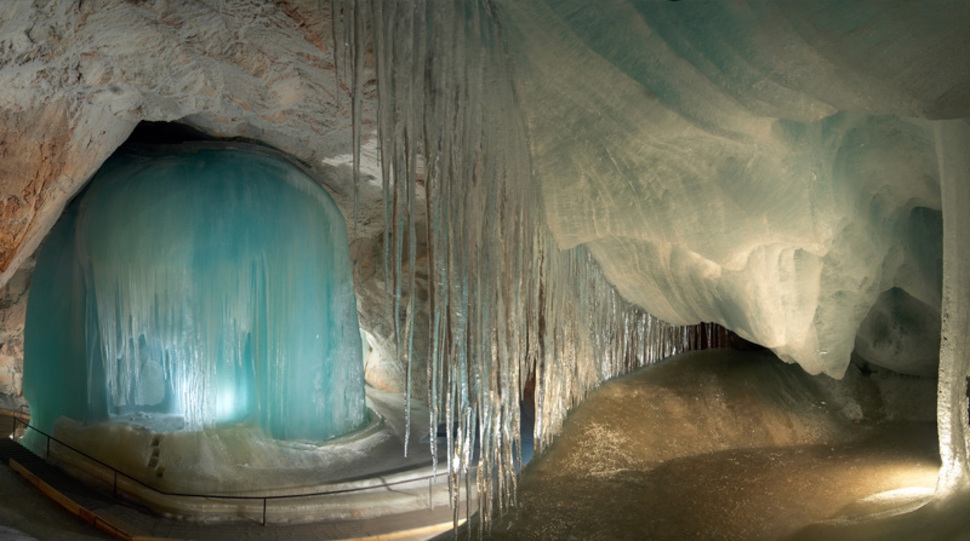
\includegraphics[height=2.8cm,width=1\textwidth,keepaspectratio]{surface_types/ice.png}\\
        \caption{Ледяная пещера}
        \label{fig:surface_types/ice}
    \end{subfigure}
  
    \begin{subfigure}[b]{0.3\textwidth}
        \centering
        \begin{tikzpicture}
            % Include the image in a node
            \node [above right, inner sep=0] (image) at (0,0)
            {\centering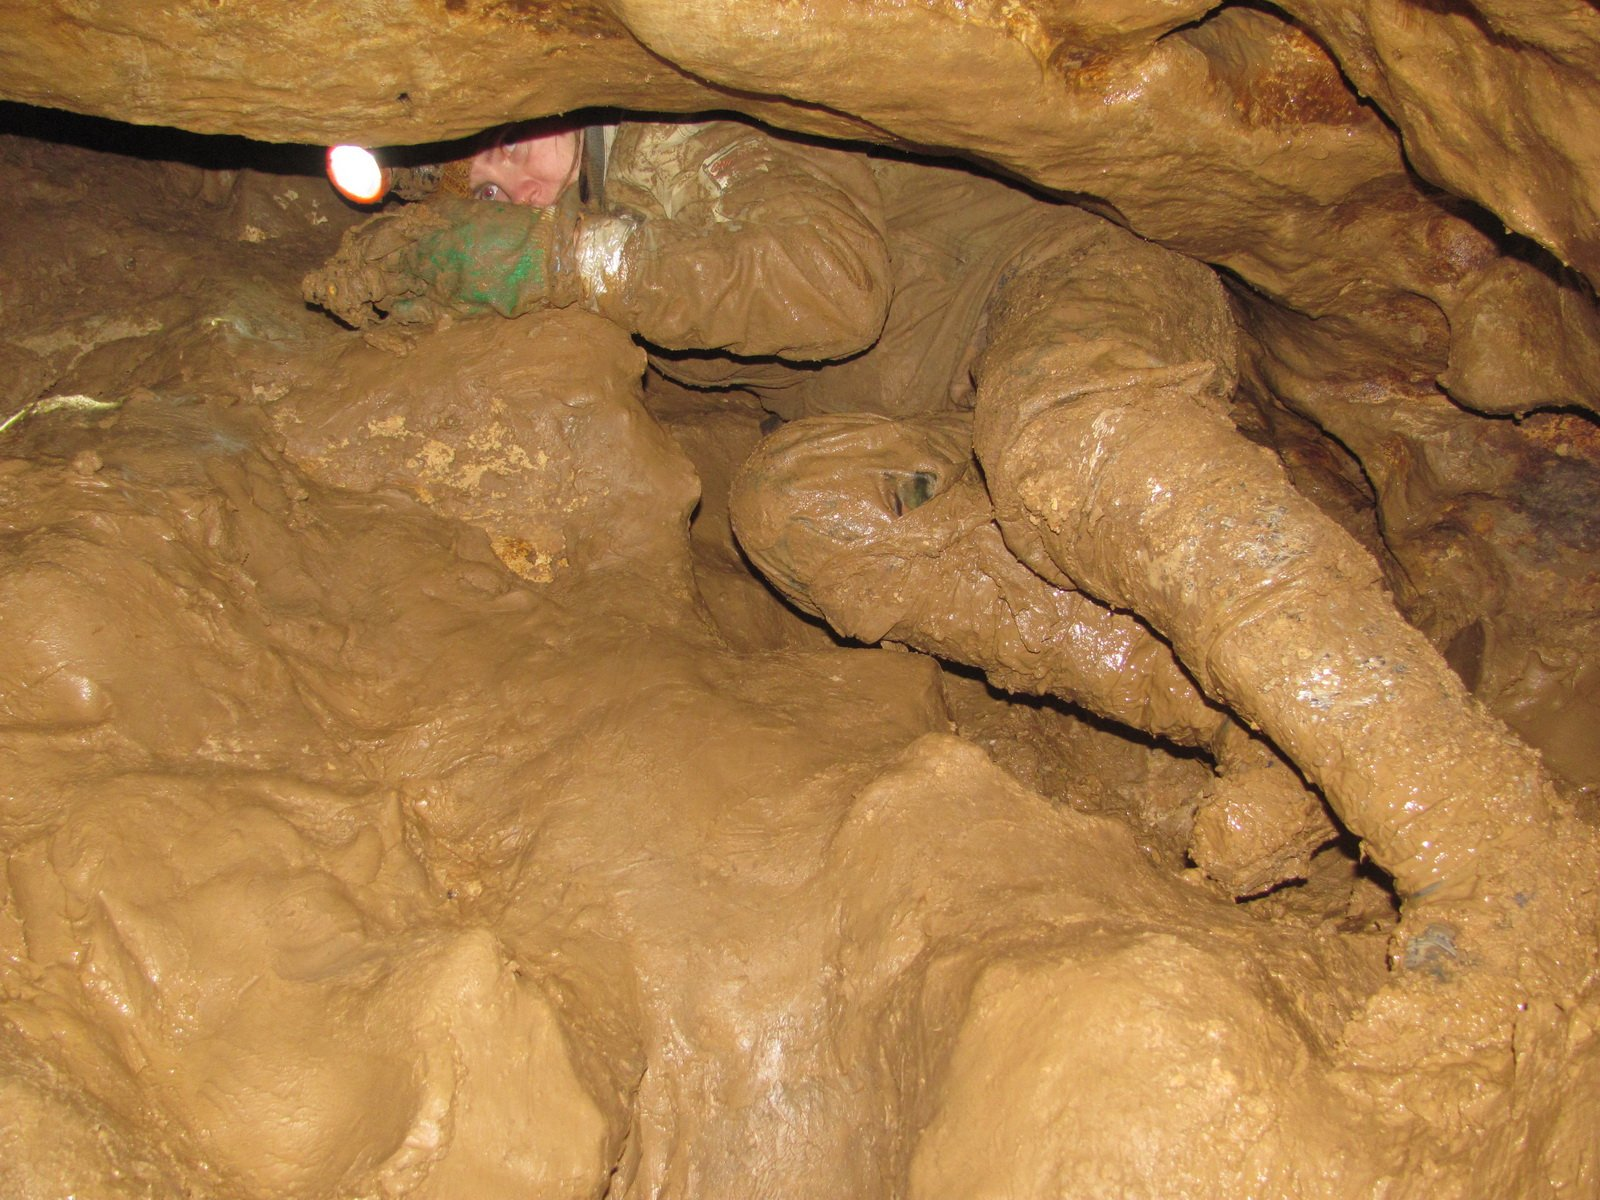
\includegraphics[height=2.8cm,width=1\textwidth,keepaspectratio]{surface_types/clay.jpg}};
            % Create scope with normalized axes
            \begin{scope}[
                    x={($ 0.1*(image.south east)$)},
                    y={($ 0.1*(image.north west)$)}]
                % Grid and axes' labels
                % \draw[lightgray,step=1] (image.south west) grid (image.north east);
                % \foreach \x in {0,1,...,10} { \node [below] at (\x,0) {\x}; }
                % \foreach \y in {0,1,...,10} { \node [left] at (0,\y) {\y};}
                % Labels
                \draw[stealth-, very thick,green] (6,8) -- ++(1,1)
                node[rounded corners=3pt,right,black,fill=white]{\tiny Человек};
            \end{scope}
        \end{tikzpicture}
        \caption{Глина}
        \label{fig:surface_types/clay.jpg}
    \end{subfigure}
    \hfill
    \begin{subfigure}[b]{0.3\textwidth}
        \centering
        \begin{tikzpicture}
            % Include the image in a node
            \node [above right, inner sep=0] (image) at (0,0)
            {\centering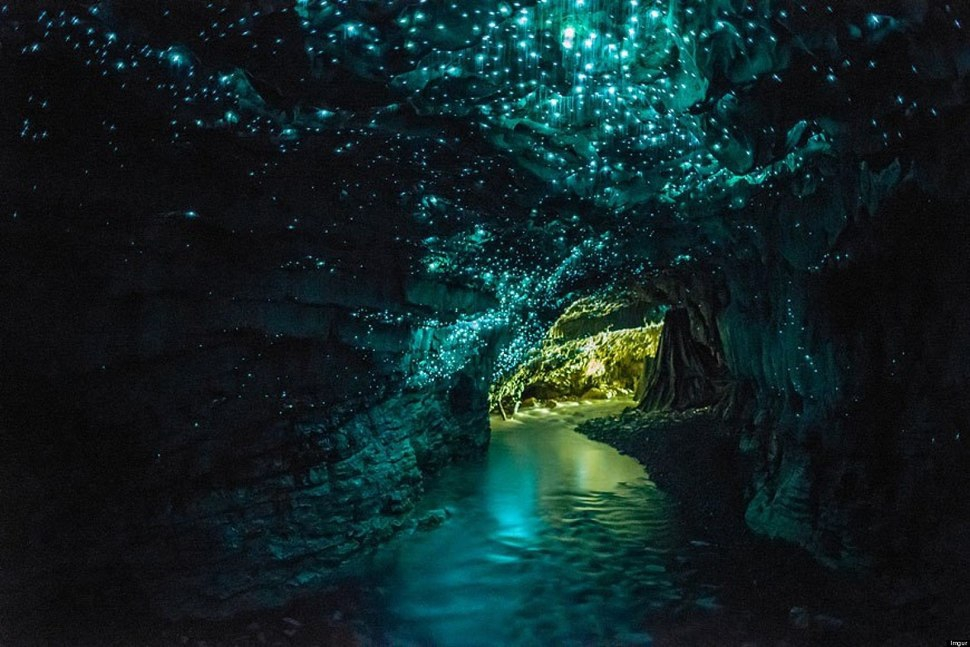
\includegraphics[height=2.8cm,width=1\textwidth,keepaspectratio]{surface_types/splash.png}};
            % Create scope with normalized axes
            \begin{scope}[
                    x={($ 0.1*(image.south east)$)},
                    y={($ 0.1*(image.north west)$)}]
                % Grid and axes' labels
                % \draw[lightgray,step=1] (image.south west) grid (image.north east);
                % \foreach \x in {0,1,...,10} { \node [below] at (\x,0) {\x}; }
                % \foreach \y in {0,1,...,10} { \node [left] at (0,\y) {\y};}
  
                % Labels
                \draw[stealth-, very thick,green] (5,2) -- ++(-2,+1)
                node[rounded corners=3pt,left,black,fill=white]{\tiny Лужа};
            \end{scope}
        \end{tikzpicture}
        \caption{Пещера, заполненная водой по~колено}
        \label{fig:surface_types/splash.png}
    \end{subfigure}
    \hfill
    \begin{subfigure}[b]{0.3\textwidth}
        \centering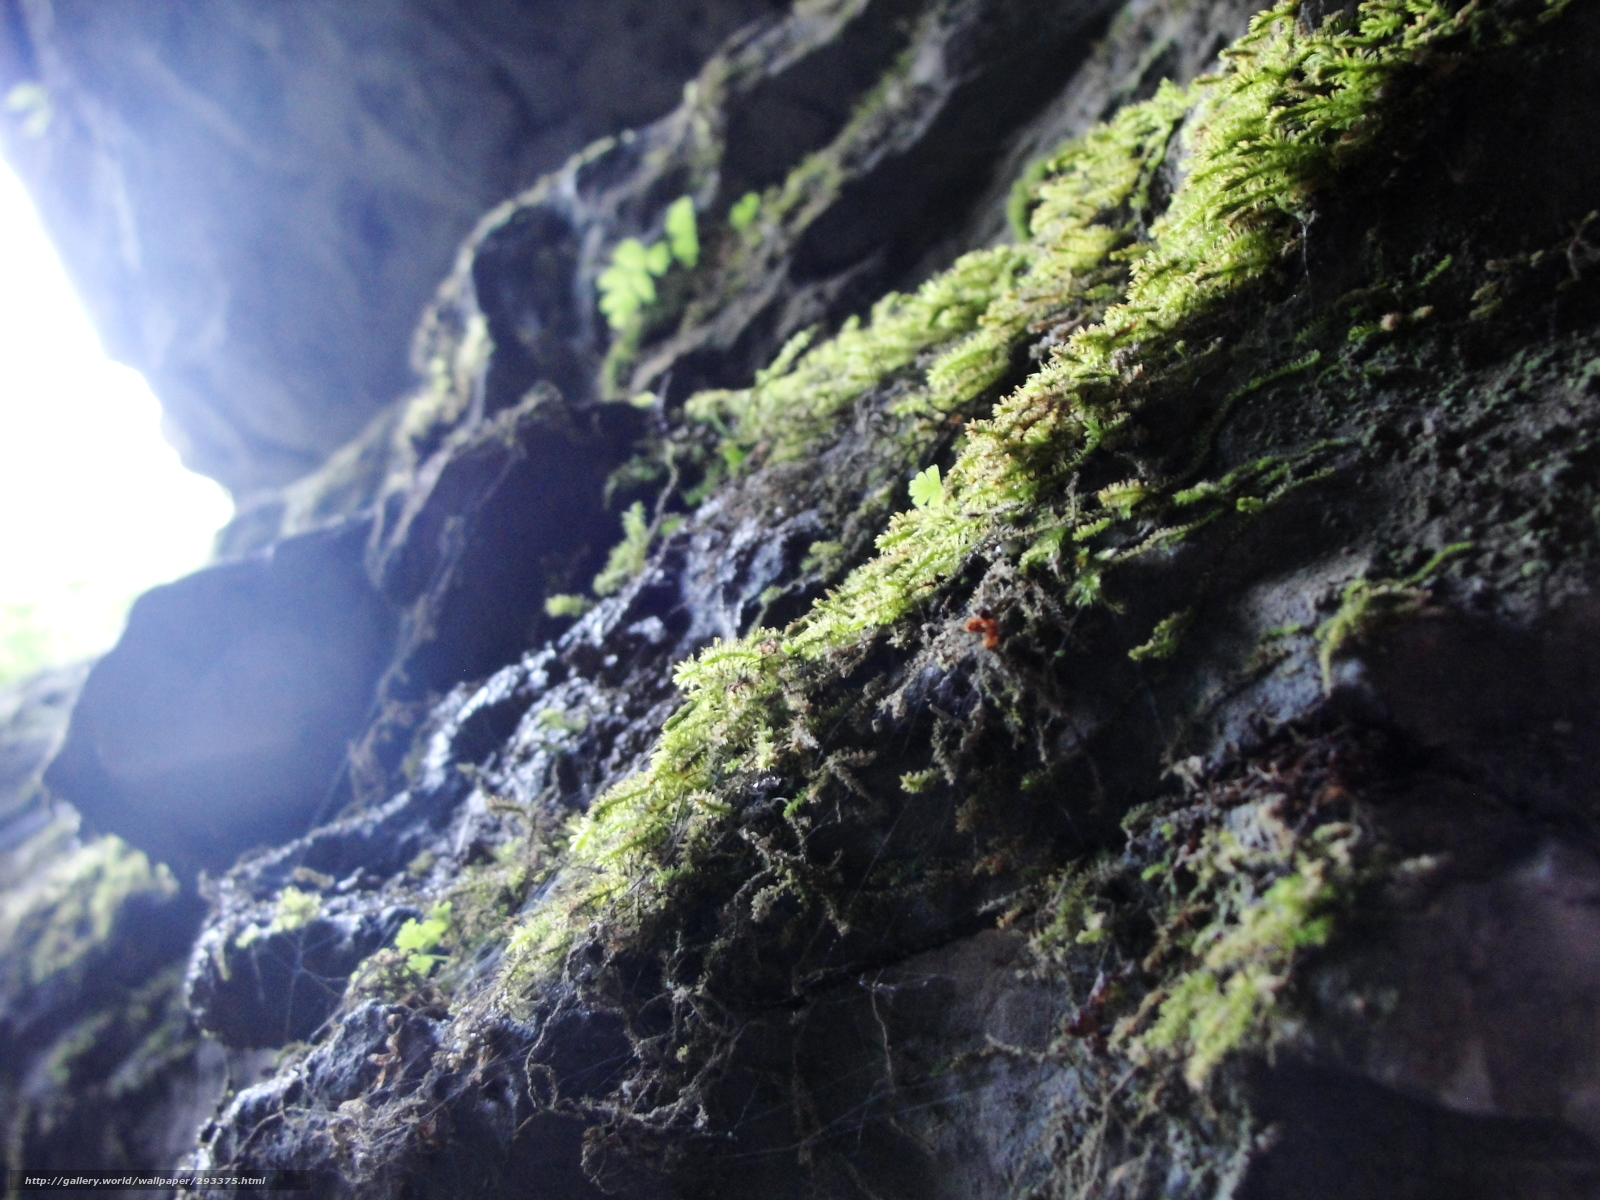
\includegraphics[height=2.8cm,width=1\textwidth,keepaspectratio]{surface_types/moss.jpg}\\
        \caption{Мох}
        \label{fig:surface_types/moss}
    \end{subfigure}
    \caption[Этот текст попадает в названия рисунков в списке рисунков]{Препятствия, встречающиеся в пещерах}\label{fig:obstacles}
  \end{figure}

Так же были рассмотрены размеры пещер, чтобы понимать необходимый запас хода, размеры робототехнического комплекса. Процентное соотношение суши/воды необходимо понимать, чтобы при разработке робота понимать какой основной функционал необходим.

\subsection{Прототипы роботов}

В диссертации рассматривались различные типы роботов. Те которые создавались специально под пещеры, космические, а так же те, которые потенциально могут быть использованы в условиях, определенных выше.

Как итог, их можно классифицировать следующим образом. Наземные роботы это шагающие, колесные, трековые и необычные. К необычным включены змеевидные, шарообразные и другие.

К летающим были отнесены защищенные дроны и дирижабли.

Но обычно для решения поставленной задачи создается робототехническая система, включающая в себя несколько роботов одного типа или комбинацию наземного и летающего роботов.

\subsection{Методы для получения полезной информации о поверхности}

Под полезной информацией рассматривается как получение самой поверхности, так и получение ее свойств. К примеру тип поверхности.

Были рассмотрены классические SLAM алгоритмы, основанные на использовании камеры, стереопары, с использованием лидара. Так же алгоритмы использующие данные с нескольких сенсоров к примеру с GPS, IMU.

Были найдены способы получения облака точек объекта с помощью касания манипулятором данного объекта. Примерное местоположение объекта определялось камерой.

Определить тип поверхности можно так же с помощью различных сенсоров: визуально, с помощью звука, с помощью датчиков силы и с помощью нескольких сенсоров одновременно.

\subsection{Вывод}
Были найдены следующие предложенные решения:
\begin{itemize}
    \item робототехнические системы для исследования свободных пещер;
    \item Построение карты с помощью лидаров и камер;
    \item Получение конечно элементной сетки с помощью тактильного очувствления манипулятором.
\end{itemize}

Таким образом, поставленная задача является новой и не была решена до этого.